% ============================================================
%  DSMarket --- Trabajo de Fin de M\'aster
%  M\'aster en Data Science & AI --- Nuclio Digital School
%  Compilar con: pdflatex $\rightarrow$ biber $\rightarrow$ pdflatex $\times$ 2
%  (o simplemente "Compile" en Overleaf con LuaLaTeX / pdfLaTeX)
% ============================================================

\documentclass[12pt, a4paper, oneside]{report}

% -
\usepackage[utf8]{inputenc}
\usepackage[T1]{fontenc}
\usepackage[provide=*,spanish]{babel}

% -
\usepackage{mathpazo}
\usepackage{microtype}
\usepackage{setspace}
\onehalfspacing

% -
\usepackage[
  top=2.5cm, bottom=2.5cm,
  inner=3.0cm, outer=2.2cm,
  headheight=14.5pt
]{geometry}

% -
\usepackage{xcolor}
% Nuclio brand: yellow + black
\definecolor{nuclioblue}{RGB}{20,20,20}       % black (main brand)
\definecolor{nucliolight}{RGB}{60,60,60}      % dark gray (secondary)
\definecolor{nuclioyellow}{RGB}{255,210,0}    % Nuclio yellow
\definecolor{nucliogray}{RGB}{100,100,100}    % medium gray
\definecolor{accentorange}{RGB}{255,180,0}    % warm yellow accent
\definecolor{lightgray}{RGB}{250,250,248}     % near-white bg
\definecolor{codegreen}{RGB}{30,130,70}
\definecolor{codegray}{RGB}{110,110,120}
\definecolor{codepurple}{RGB}{130,0,130}
\definecolor{codeblue}{RGB}{0,60,180}
\definecolor{rowalt}{RGB}{255,252,225}        % pale yellow rows
\definecolor{headerblue}{RGB}{20,20,20}       % black header

% -
\usepackage{graphicx}
\usepackage{float}
\usepackage{caption}
\usepackage{subcaption}
\captionsetup{
  font=small,
  labelfont={bf,color=nuclioblue},
  skip=6pt
}

% -
\usepackage{booktabs}
\usepackage{tabularx}
\usepackage{multirow}
\usepackage{array}
\usepackage{longtable}
\usepackage{colortbl}
\newcolumntype{L}[1]{>{\raggedright\arraybackslash}p{#1}}
\newcolumntype{C}[1]{>{\centering\arraybackslash}p{#1}}
\newcolumntype{R}[1]{>{\raggedleft\arraybackslash}p{#1}}

% -
\usepackage{listings}
\lstdefinestyle{pythonstyle}{
  language=Python,
  basicstyle=\ttfamily\footnotesize,
  keywordstyle=\bfseries\color{codeblue},
  commentstyle=\itshape\color{codegreen},
  stringstyle=\color{codepurple},
  numberstyle=\tiny\color{codegray},
  numbers=left,
  numbersep=8pt,
  stepnumber=1,
  breaklines=true,
  breakatwhitespace=false,
  showstringspaces=false,
  frame=single,
  framesep=4pt,
  rulecolor=\color{nuclioblue!40},
  backgroundcolor=\color{lightgray},
  xleftmargin=16pt,
  xrightmargin=4pt,
  tabsize=4,
  captionpos=b
}
\lstdefinestyle{pseudostyle}{
  basicstyle=\ttfamily\footnotesize,
  numberstyle=\tiny\color{codegray},
  numbers=none,
  breaklines=true,
  frame=single,
  framesep=4pt,
  rulecolor=\color{nuclioblue!30},
  backgroundcolor=\color{lightgray},
  xleftmargin=10pt,
  xrightmargin=4pt,
}
\lstset{style=pythonstyle}
\lstset{
  literate=
    {á}{{\'a}}1 {é}{{\'e}}1 {í}{{\'i}}1 {ó}{{\'o}}1 {ú}{{\'u}}1
    {Á}{{\'A}}1 {É}{{\'E}}1 {Í}{{\'I}}1 {Ó}{{\'O}}1 {Ú}{{\'U}}1
    {ñ}{{\~n}}1 {Ñ}{{\~N}}1
}

% -
\usepackage{tcolorbox}
\tcbuselibrary{skins, breakable, theorems}

\tcbset{
  canvasbox/.style={
    enhanced,
    breakable,
    colback=lightgray,
    colframe=nuclioblue,
    fonttitle=\bfseries\small\color{white},
    title style={left color=nuclioblue, right color=nucliolight},
    attach boxed title to top left={yshift=-2mm, xshift=6mm},
    boxed title style={
      colback=nuclioblue, colframe=nuclioblue,
      sharp corners, rounded corners=northeast
    },
    arc=4pt,
    boxrule=0.8pt,
    top=6pt, bottom=6pt, left=8pt, right=8pt
  }
}

\tcbset{
  insightbox/.style={
    enhanced,
    colback=nucliolight!8,
    colframe=nucliolight!60,
    fonttitle=\bfseries\small\color{nuclioblue},
    coltitle=nuclioblue,
    attach boxed title to top left={yshift=-2mm, xshift=6mm},
    boxed title style={colback=nucliolight!15, colframe=nucliolight!60, sharp corners},
    arc=3pt, boxrule=0.7pt,
    top=5pt, bottom=5pt, left=8pt, right=8pt
  }
}

% -
\usepackage{fancyhdr}
\pagestyle{fancy}
\fancyhf{}
\fancyhead[LE]{\small\color{nucliogray}\leftmark}
\fancyhead[RO]{\small\color{nucliogray}\rightmark}
\fancyfoot[C]{\small\color{nucliogray}\thepage}
\renewcommand{\headrulewidth}{0.4pt}
\renewcommand{\headrule}{\hbox to\headwidth{\color{nuclioblue}\leaders\hrule height \headrulewidth\hfill}}

% -
\usepackage{titlesec}

\titleformat{\chapter}[display]
  {\normalfont\bfseries\huge\color{nuclioblue}}
  {\filleft\small\color{nucliogray}\MakeUppercase{\chaptertitlename}\hspace{0.5em}
   \fontsize{50}{50}\selectfont\color{nuclioyellow}\thechapter}
  {-10pt}
  {\color{nuclioyellow}\hrule height 2pt\vspace{6pt}}

\titleformat{\section}
  {\normalfont\bfseries\large\color{nuclioblue}}
  {\thesection}{0.8em}{}

\titleformat{\subsection}
  {\normalfont\bfseries\normalsize\color{nucliolight}}
  {\thesubsection}{0.7em}{}

\titleformat{\subsubsection}
  {\normalfont\bfseries\small\color{nucliogray}}
  {\thesubsubsection}{0.6em}{}

\titlespacing*{\chapter}{0pt}{-20pt}{20pt}
\titlespacing*{\section}{0pt}{16pt}{6pt}
\titlespacing*{\subsection}{0pt}{12pt}{4pt}

% -
\usepackage{hyperref}
\hypersetup{
  colorlinks = true,
  linkcolor  = nuclioblue,
  citecolor  = accentorange,
  urlcolor   = nucliolight,
  pdftitle   = {DSMarket: Sistema de Predicci\'on de Demanda y Optimizaci\'on del Abastecimiento},
  pdfauthor  = {Gabriela Alberico, Jorge Silva, Robert Tunzi, Matias Lannes, Alexis Labrador},
  bookmarksnumbered = true
}

% -

% -
\usepackage{amsmath, amssymb}

% -
\usepackage{enumitem}
\usepackage{mdframed}
\usepackage{parskip}
\setlength{\parskip}{6pt}
\usepackage{afterpage}

% -
\newcommand{\kpi}[1]{\textbf{\color{accentorange}#1}}
\newcommand{\code}[1]{\texttt{\small\color{codeblue}#1}}
\newcommand{\dataset}[1]{\texttt{\footnotesize\color{codepurple}#1}}
\newcommand{\model}[1]{\textbf{\color{nucliolight}#1}}
\newcommand{\metric}[1]{\textbf{\color{accentorange}#1}}

\usepackage{tikz}
\usetikzlibrary{arrows.meta, positioning, shapes.geometric}

% -
%  DOCUMENT
% -
\begin{document}

% -
%  PORTADA
% -
\begin{titlepage}
\pagecolor{nuclioblue}

\begin{center}

\vspace*{0.8cm}

{%
  \fontsize{26}{32}\bfseries\color{white}%
  NUCLIO \textcolor{nuclioyellow}{DIGITAL SCHOOL}%
}\\[0.15cm]
{\small\color{white!75} M\'aster en Data Science \& Artificial Intelligence}\\[0.1cm]
{\color{nuclioyellow}\rule{0.7\textwidth}{1pt}}

\vspace{1.4cm}

{\small\color{white!80}\MakeUppercase{Trabajo de Fin de M\'aster}}\\[0.4cm]
{\color{nuclioyellow}\rule{0.7\textwidth}{2pt}}\\[0.6cm]

{\fontsize{24}{30}\bfseries\color{white}
  DSMarket: Sistema de Predicci\'on\\[0.2cm]
  de Demanda y Optimizaci\'on del\\[0.2cm]
  Abastecimiento mediante\\[0.2cm]
  Machine Learning
}\\[0.6cm]

{\color{nuclioyellow}\rule{0.7\textwidth}{2pt}}

\vspace{1.4cm}

\begin{tabular}{rl}
  \color{white!70}Autores: & \color{white}Gabriela Alberico, Jorge Silva,\\
                           & \color{white}Robert Tunzi, Mat\'{\i}as Lannes,\\
                           & \color{white}Alexis Labrador \\[4pt]
  \color{white!70}Grupo: & \color{white}2 --- DSCESP 0925 \\[4pt]
  \color{white!70}Tutor: & \color{white}Mat\'{\i}as Jos\'e Hermida \\
                         & \color{white!60}\small\itshape Senior Data Scientist, CaixaBank BI \\[4pt]
  \color{white!70}Per\'{\i}odo: & \color{white}Septiembre 2025 -- Abril 2026 \\[4pt]
  \color{white!70}Defensa: & \color{white}Abril de 2026 \\
\end{tabular}

\vfill

{\small\color{white!50} Versi\'on 1.0 --- Marzo 2026}

\end{center}
\end{titlepage}
\nopagecolor

% -
%  RESUMEN EJECUTIVO
% -
\chapter*{Resumen Ejecutivo}
\addcontentsline{toc}{chapter}{Resumen Ejecutivo}
\markboth{Resumen Ejecutivo}{}

\textbf{DSMarket} es una cadena de supermercados que opera 10 tiendas en tres ciudades de Estados Unidos (Nueva York, Boston y Filadelfia) con un cat\'alogo de m\'as de 3.000 productos. La ineficiencia en la gesti\'on manual del inventario genera p\'erdidas por \textit{stockouts} (ventas perdidas) y por exceso de stock (capital inmovilizado), motivando el desarrollo de este proyecto.

El presente Trabajo de Fin de M\'aster desarrolla un \textbf{sistema \textit{end-to-end} de predicci\'on de demanda y optimizaci\'on del abastecimiento} para DSMarket, aplicando t\'ecnicas de Machine Learning sobre datos hist\'oricos de ventas del per\'{\i}odo 2011--2016 (\textasciitilde58,3 millones de registros a granularidad \'{\i}tem-tienda-d\'{\i}a).

La metodolog\'{\i}a comprende cinco fases diferenciadas:

\begin{enumerate}[leftmargin=*, noitemsep]
  \item \textbf{An\'alisis exploratorio (EDA) y limpieza}, con seis hallazgos accionables sobre patrones geogr\'aficos, semanales y la elasticidad precio-demanda.
  \item \textbf{Feature Engineering}, con 28 variables construidas a partir de lags temporales, estad\'{\i}sticos de ventana deslizante y features de precio.
  \item \textbf{Clustering} de productos (k=5) y tiendas (k=3) mediante K-Means, identificando segmentos con comportamientos de demanda diferenciados.
  \item \textbf{Modelizaci\'on predictiva}, comparando Baseline (media m\'ovil 28 d\'{\i}as), Ridge, Random Forest, CatBoost, LightGBM y \model{XGBoost}, con optimizaci\'on bayesiana de hiperpar\'ametros mediante Optuna.
  \item \textbf{Sistema de abastecimiento autom\'atico}, que genera \'ordenes de reposici\'on semanales con clasificaci\'on de prioridad (ALTA/NORMAL).
\end{enumerate}

El modelo final (\model{XGBoost} post-Optuna) obtiene un \metric{RMSE = 1,8994} en el conjunto de validaci\'on, representando una \kpi{mejora del 13,1\%} sobre el baseline (RMSE = 2,18), superando el objetivo m\'{\i}nimo del 5\% establecido en los objetivos del proyecto.

\bigskip
\noindent\textbf{Palabras clave:} predicci\'on de demanda, retail forecasting, XGBoost, Gradient Boosting, Optuna, K-Means clustering, sistema de abastecimiento, MLOps, series temporales, M5 Forecasting.

% -
%  \'INDICE
% -
\tableofcontents
\clearpage
\listoftables
\addcontentsline{toc}{chapter}{\'Indice de tablas}
\clearpage

% -
%  CAP\'ITULO 1 --- INTRODUCCI\'ON
% -
\chapter{Introducci\'on}

\section{Contexto del proyecto}

El presente Trabajo de Fin de M\'aster se desarrolla en el marco del programa \textbf{M\'aster en Data Science \& AI} de \textbf{Nuclio Digital School}, bajo la modalidad de proyecto Tipo~1 (\textit{Role-play}) orientado al sector \textit{Retail}. El escenario propuesto es el de \textbf{DSMarket}, una cadena de supermercados con presencia en tres ciudades de Estados Unidos (Nueva York, Boston y Filadelfia) que opera 10 tiendas y gestiona un cat\'alogo de m\'as de 3.000 productos.

La direcci\'on de la compa\~n\'{\i}a, representada por sus ejecutivos de nivel C (Paul, CFO, y Michelle, CDO), ha solicitado al equipo de Data Science el desarrollo de un sistema de inteligencia que permita \textbf{anticipar la demanda futura} de cada producto en cada tienda. El problema central es la ineficiencia en la gesti\'on del inventario: DSMarket incurre en p\'erdidas por \textbf{\textit{stockouts}} (productos agotados que generan ventas perdidas) y por \textbf{exceso de stock} (capital inmovilizado en productos que no se venden con la velocidad esperada).

La gesti\'on manual del inventario, basada en criterios subjetivos o en medias hist\'oricas simples, no es capaz de capturar la complejidad de los patrones de demanda, que var\'{\i}an seg\'un el d\'{\i}a de la semana, el mes del a\~no, los eventos especiales (SuperBowl, Thanksgiving, New Year, etc.) y las fluctuaciones de precio.

\section{Motivaci\'on}

El presente proyecto aplica t\'ecnicas de \textbf{Machine Learning supervisado} sobre datos hist\'oricos de ventas para construir un modelo predictivo que supere al baseline y, a partir de sus predicciones, genere autom\'aticamente \textbf{\'ordenes de reposici\'on} para cada tienda. Este sistema representa el paso de una gesti\'on \textit{reactiva} (reponer cuando el stock es bajo) a una gesti\'on \textbf{proactiva y basada en datos} (reponer antes de que ocurra el \textit{stockout}).

\begin{tcolorbox}[canvasbox, title={Motivaci\'on del proyecto}]
El sector \textit{retail} enfrenta un desaf\'{\i}o estructural: los modelos tradicionales de gesti\'on de inventario no capturan la heterogeneidad de la demanda a nivel de producto-tienda-d\'{\i}a. Un modelo de Machine Learning entrenado sobre 58 millones de registros hist\'oricos puede capturar esas interacciones complejas y traducirlas en \'ordenes de reposici\'on concretas, reduciendo tanto el riesgo de \textit{stockout} como el coste del exceso de inventario.
\end{tcolorbox}

\section{Estructura del documento}

Este documento se organiza en cuatro grandes bloques:

\begin{enumerate}[leftmargin=*, noitemsep]
  \item \textbf{Objetivos}: qu\'e se pretende lograr con el proyecto.
  \item \textbf{Metodolog\'{\i}a}: descripci\'on de los datos, las t\'ecnicas aplicadas y las decisiones metodol\'ogicas tomadas.
  \item \textbf{Resultados y Conclusiones}: presentaci\'on de los resultados obtenidos, las variables m\'as influyentes y las conclusiones derivadas del an\'alisis.
  \item \textbf{Referencias bibliogr\'aficas}: referencias a los trabajos y herramientas utilizados.
  \item \textbf{Anexo --- ML Canvas}: descomposici\'on estructurada del sistema mediante el marco \textit{Machine Learning Canvas}.
\end{enumerate}

% -
%  CAP\'ITULO 2 --- OBJETIVOS
% -
\chapter{Objetivos}

\section{Objetivo general}

Desarrollar un sistema \textit{end-to-end} de \textbf{predicci\'on de demanda y optimizaci\'on del abastecimiento} para DSMarket, que permita a la direcci\'on tomar decisiones informadas sobre la gesti\'on del inventario, reduciendo los costes operativos y mejorando el nivel de servicio al cliente.

\section{Objetivos espec\'{\i}ficos}

La Tabla~\ref{tab:objetivos} resume los seis objetivos espec\'{\i}ficos del proyecto, junto con sus indicadores de \'exito.

\begin{longtable}{C{0.7cm} L{4.8cm} L{6.8cm}}
  \caption{Objetivos espec\'{\i}ficos del proyecto DSMarket}
  \label{tab:objetivos}\\
  \toprule
  \rowcolor{headerblue}
  {\color{white}\textbf{\#}} &
  {\color{white}\textbf{Objetivo}} &
  {\color{white}\textbf{Indicador de \'exito}} \\
  \midrule
  \endfirsthead
  \multicolumn{3}{c}{\small\itshape (continuaci\'on de la Tabla \ref{tab:objetivos})}\\
  \toprule
  \rowcolor{headerblue}
  {\color{white}\textbf{\#}} &
  {\color{white}\textbf{Objetivo}} &
  {\color{white}\textbf{Indicador de \'exito}} \\
  \midrule
  \endhead
  \bottomrule
  \endlastfoot
  \rowcolor{white}
  \textbf{O1} &
  Realizar un an\'alisis exploratorio completo (EDA) que identifique patrones de demanda, estacionalidad y anomal\'{\i}as &
  Al menos 5 hallazgos de negocio accionables documentados y visualizados \\
  \rowcolor{rowalt}
  \textbf{O2} &
  Segmentar productos y tiendas mediante clustering para identificar grupos con comportamientos diferenciados &
  \textit{Silhouette score} maximizado para cada nivel de granularidad, con interpretaci\'on de negocio clara por cl\'uster \\
  \rowcolor{white}
  \textbf{O3} &
  Construir un modelo de predicci\'on de ventas que supere estad\'{\i}sticamente al baseline (media m\'ovil 28 d\'{\i}as) en RMSE &
  Mejora m\'{\i}nima del 5\% en RMSE sobre el baseline en el conjunto de test \\
  \rowcolor{rowalt}
  \textbf{O4} &
  Optimizar los hiperpar\'ametros del modelo ganador mediante b\'usqueda bayesiana (Optuna) &
  RMSE en validaci\'on $\leq$ RMSE del modelo inicial sin optimizar \\
  \rowcolor{white}
  \textbf{O5} &
  Desarrollar un sistema automatizado de reposici\'on de inventario que consuma las predicciones del modelo &
  Sistema capaz de generar \'ordenes de reposici\'on para cualquier combinaci\'on tienda-producto con clasificaci\'on de prioridad (ALTA/NORMAL) \\
  \rowcolor{rowalt}
  \textbf{O6} &
  Exportar las predicciones y m\'etricas a Power~BI para su visualizaci\'on y presentaci\'on ejecutiva &
  \textit{Dashboard} funcional con al menos 4 vistas diferenciadas \\
\end{longtable}

\section{Finalidad del proyecto}

La finalidad \'ultima de este proyecto es demostrar que las t\'ecnicas de Data Science pueden \textbf{crear valor de negocio tangible} en el sector \textit{Retail}. La combinaci\'on de an\'alisis exploratorio, clustering, predicci\'on y sistema de abastecimiento proporciona a DSMarket una soluci\'on integral que no solo predice la demanda, sino que \textbf{traduce esas predicciones en acciones concretas}: las \'ordenes de reposici\'on.

Adicionalmente, el proyecto sirve como demostraci\'on pr\'actica de los conocimientos adquiridos a lo largo del M\'aster en Data Science, cubriendo el ciclo completo de un proyecto de ML: desde la obtenci\'on y limpieza de datos hasta la toma de decisiones basada en el modelo, incluyendo una \textbf{propuesta detallada de puesta en producci\'on} (secci\'on MLOps) que describe los pasos de despliegue, monitoreo y reentrenamiento que se seguir\'{\i}an en un entorno real.

% -
%  CAP\'ITULO 3 --- METODOLOG\'IA
% -
\chapter{Metodolog\'{\i}a Empleada}

\section{Descripci\'on del dataset}

El proyecto parte de tres fuentes de datos internas de DSMarket, correspondientes al per\'{\i}odo \textbf{29 de enero de 2011 -- 24 de abril de 2016} (1.913 d\'{\i}as).

\begin{table}[H]
  \centering
  \caption{Fuentes de datos utilizadas en el proyecto}
  \label{tab:datasets}
  \begin{tabularx}{\textwidth}{L{3.2cm} L{5.5cm} L{4.5cm}}
    \toprule
    \rowcolor{headerblue}
    {\color{white}\textbf{Dataset}} &
    {\color{white}\textbf{Descripci\'on}} &
    {\color{white}\textbf{Dimensiones}} \\
    \midrule
    \rowcolor{white}
    \dataset{item\_sales.csv} &
    Ventas diarias por producto-tienda en formato \textit{wide} &
    30.490 filas $\times$ 1.920 columnas \\
    \rowcolor{rowalt}
    \dataset{daily\_calendar\_with\_events.csv} &
    Calendario con fechas y eventos especiales &
    1.913 filas $\times$ 5 columnas \\
    \rowcolor{white}
    \dataset{item\_prices.csv} &
    Precios semanales por producto-tienda &
    $\sim$7 millones de filas $\times$ 5 columnas \\
    \bottomrule
  \end{tabularx}
\end{table}

El dataset de ventas original tiene formato \textbf{\textit{wide}}: cada fila es una combinaci\'on producto-tienda y cada columna representa un d\'{\i}a (\code{d\_1}, \code{d\_2}, \ldots, \code{d\_1913}). Mediante una operaci\'on de \textit{unpivot} (transformaci\'on \textit{wide}$\rightarrow$\textit{long} con \code{melt}), se convierte en un formato donde cada fila representa exactamente un registro (\textit{item}, \textit{store}, d\'{\i}a)$\rightarrow$ventas. Esto se denomina \textbf{granularidad \'{\i}tem-tienda-d\'{\i}a} e implica que cada fila responde a la pregunta: \textit{``?`cu\'antas unidades vendi\'o este producto concreto, en esta tienda concreta, en este d\'{\i}a concreto?''}. Tras la transformaci\'on, el dataset consolidado contiene aproximadamente \textbf{58,3 millones de registros}.

\begin{tcolorbox}[insightbox, title={Caracter\'{\i}sticas del \'ambito de an\'alisis}]
\begin{itemize}[noitemsep, leftmargin=*]
  \item \textbf{3.049 productos \'unicos} organizados en 3 categor\'{\i}as (SUPERMARKET, ACCESSORIES, HOME\_\&\_GARDEN) y 7 departamentos.
  \item \textbf{10 tiendas} en 3 ciudades: New York, Boston y Philadelphia.
  \item \textbf{Variable objetivo}: \code{sales} --- ventas diarias en unidades, con distribuci\'on asim\'etrica positiva y cola larga.
\end{itemize}
\end{tcolorbox}

\section{An\'alisis Exploratorio de Datos (EDA) y Limpieza}

\subsection{Limpieza de datos}

El proceso de limpieza se aplic\'o de forma diferenciada a cada fuente de datos.

\subsubsection{Sales data}
No se encontraron valores nulos ni duplicados. Los valores \code{0} en las columnas de ventas son datos reales: representan d\'{\i}as en que un producto no se vendi\'o, no registros faltantes. Se aplic\'o limpieza de espacios en los identificadores de texto.

\subsubsection{Calendar data}
La columna \code{event} conten\'{\i}a 1.887 \textit{strings} vac\'{\i}os (d\'{\i}as sin evento especial). Estos se convirtieron correctamente a \code{NaN} en lugar de dejarse como \textit{strings} vac\'{\i}os, ya que la ausencia de evento es informaci\'on, no un dato faltante. Adicionalmente se crearon \textit{features} temporales derivadas: \code{year}, \code{month}, \code{day}, \code{quarter}, \code{week\_of\_year}, \code{is\_weekend} e \code{is\_event}.

\subsubsection{Prices data}
Se detectaron 243.920 valores nulos (3,50\%) en la columna \code{yearweek}, distribuidos uniformemente entre todos los productos y tiendas. Se imputaron mediante la \textbf{mediana por grupo} (\code{item} + \code{store\_code}), preservando el patr\'on de precios espec\'{\i}fico de cada producto en cada tienda. Se verific\'o que no existen precios negativos ni cero. Se confirm\'o la consistencia del cat\'alogo: los 3.049 productos de ventas tienen correspondencia exacta en la tabla de precios. No se encontraron duplicados en ninguna de las tres fuentes.

\subsection{Hallazgos del EDA}

\begin{tcolorbox}[canvasbox, title={Hallazgo 1 --- Liderazgo geogr\'afico de New York}]
New York concentra el mayor volumen de ventas de las tres ciudades. Boston y Filadelfia presentan cifras muy similares entre s\'{\i}. \textbf{Implicaci\'on de negocio}: las pol\'{\i}ticas de stock y reposici\'on deben priorizarse por ciudad, no tratarse de forma uniforme.
\end{tcolorbox}

\begin{tcolorbox}[canvasbox, title={Hallazgo 2 --- Efecto fin de semana consistente y cuantificado}]
El s\'abado y el domingo generan entre un \textbf{27--33\% m\'as de ventas} que los d\'{\i}as laborales en todas las ciudades. El mi\'ercoles es el d\'{\i}a de menor actividad (``punto muerto'' semanal). \textbf{Implicaci\'on}: los pedidos de reposici\'on deben planificarse para que el stock llegue antes del jueves.
\end{tcolorbox}

\begin{tcolorbox}[canvasbox, title={Hallazgo 3 --- SUPERMARKET es el motor del negocio}]
La categor\'{\i}a SUPERMARKET representa el \textbf{68,7\% de las ventas totales}. HOME \& GARDEN aporta el 22\% y ACCESSORIES el 9,3\%. Dentro de SUPERMARKET, el departamento SUPERMARKET\_3 domina de forma clara. \textbf{Implicaci\'on}: cualquier fallo de stock en SUPERMARKET tiene un impacto desproporcionado en la facturaci\'on global.
\end{tcolorbox}

\begin{tcolorbox}[canvasbox, title={Hallazgo 4 --- El pico de 2013 fue provocado por bajada de precios}]
El an\'alisis conjunto de ventas y precios revela que el gran pico hist\'orico (septiembre 2013) coincide exactamente con una ca\'{\i}da dr\'astica de precios en los productos l\'{\i}deres. \textbf{Implicaci\'on}: la elasticidad precio-demanda es un \textit{driver} real en este negocio, y las variables de precio son \textit{features} relevantes para el modelo.
\end{tcolorbox}

\begin{tcolorbox}[canvasbox, title={Hallazgo 5 --- Impacto diferenciado de los eventos especiales}]
SuperBowl (\textbf{+15,36\%} sobre la media) y Easter (\textbf{+12,38\%}) disparan las ventas. Thanksgiving las reduce dr\'asticamente (\textbf{$-$40,21\%}), posiblemente por cierre de tiendas. \textbf{Implicaci\'on}: el calendario de eventos es una variable predictiva de alto valor y debe incorporarse al modelo.
\end{tcolorbox}

\begin{tcolorbox}[canvasbox, title={Hallazgo 6 --- Fuerte autocorrelaci\'on en lag~1 (ACF $\approx$ 0,78)}]
Las ventas de ayer son el predictor individual m\'as potente de las ventas de hoy. El test Augmented Dickey-Fuller confirma que la serie es \textbf{estacionaria} ($p$-value = 0,0008), por lo que no se requieren transformaciones adicionales (diferenciaci\'on, logaritmos). \textbf{Implicaci\'on metodol\'ogica}: los modelos de Gradient Boosting con \textit{lag features} son la aproximaci\'on correcta para este problema.
\end{tcolorbox}

\section{Feature Engineering}

Se construy\'o un \textbf{pipeline de \textit{feature engineering}} (\code{feature\_engineering\_pipeline}) utilizando \code{sklearn.pipeline.Pipeline} y \code{sklearn.preprocessing.FunctionTransformer}. Las variables generadas se agrupan en cuatro familias.

\subsection{Features de lag (memoria temporal)}

\begin{table}[H]
  \centering
  \caption{Features de lag y estad\'{\i}sticos de ventana deslizante}
  \label{tab:lag_features}
  \begin{tabularx}{\textwidth}{L{3.8cm} X}
    \toprule
    \rowcolor{headerblue}
    {\color{white}\textbf{Feature}} & {\color{white}\textbf{Descripci\'on}} \\
    \midrule
    \rowcolor{white}   \code{sales\_lag\_1}           & Ventas del d\'{\i}a anterior \\
    \rowcolor{rowalt}  \code{sales\_lag\_7}           & Ventas hace 7 d\'{\i}as (mismo d\'{\i}a de la semana pasada) \\
    \rowcolor{white}   \code{sales\_lag\_14}          & Ventas hace 14 d\'{\i}as \\
    \rowcolor{rowalt}  \code{sales\_lag\_21}          & Ventas hace 21 d\'{\i}as \\
    \rowcolor{white}   \code{sales\_lag\_28}          & Ventas hace 28 d\'{\i}as \\
    \rowcolor{rowalt}  \code{rolling\_mean\_7}        & Media m\'ovil de 7 d\'{\i}as \\
    \rowcolor{white}   \code{rolling\_mean\_14}       & Media m\'ovil de 14 d\'{\i}as \\
    \rowcolor{rowalt}  \code{rolling\_mean\_28}       & Media m\'ovil de 28 d\'{\i}as \\
    \rowcolor{white}   \code{rolling\_std\_7}         & Desviaci\'on est\'andar de 7 d\'{\i}as \\
    \rowcolor{rowalt}  \code{rolling\_std\_14}        & Desviaci\'on est\'andar de 14 d\'{\i}as \\
    \rowcolor{white}   \code{rolling\_std\_28}        & Desviaci\'on est\'andar de 28 d\'{\i}as \\
    \rowcolor{rowalt}  \code{rolling\_max\_28}        & M\'aximo de ventas en los \'ultimos 28 d\'{\i}as \\
    \rowcolor{white}   \code{rolling\_min\_28}        & M\'{\i}nimo de ventas en los \'ultimos 28 d\'{\i}as \\
    \bottomrule
  \end{tabularx}
\end{table}

\subsection{Features temporales}

\begin{table}[H]
  \centering
  \caption{Features temporales derivadas del calendario}
  \label{tab:temporal_features}
  \begin{tabularx}{\textwidth}{L{3.8cm} X}
    \toprule
    \rowcolor{headerblue}
    {\color{white}\textbf{Feature}} & {\color{white}\textbf{Descripci\'on}} \\
    \midrule
    \rowcolor{white}   \code{weekday\_int}     & D\'{\i}a de la semana como entero (1 = s\'abado, 2 = domingo, \ldots) \\
    \rowcolor{rowalt}  \code{day}              & D\'{\i}a del mes \\
    \rowcolor{white}   \code{week\_of\_year}   & Semana del a\~no (1--52) \\
    \rowcolor{rowalt}  \code{month}            & Mes del a\~no (1--12) \\
    \rowcolor{white}   \code{quarter}          & Trimestre del a\~no (1--4) \\
    \rowcolor{rowalt}  \code{year}             & A\~no \\
    \rowcolor{white}   \code{is\_weekend}      & Indicador binario: 1 si es s\'abado o domingo \\
    \rowcolor{rowalt}  \code{is\_event}        & Indicador binario: 1 si hay evento especial ese d\'{\i}a \\
    \bottomrule
  \end{tabularx}
\end{table}

\subsection{Features de precio}

\begin{table}[H]
  \centering
  \caption{Features de precio y sus variaciones}
  \label{tab:price_features}
  \begin{tabularx}{\textwidth}{L{3.8cm} X}
    \toprule
    \rowcolor{headerblue}
    {\color{white}\textbf{Feature}} & {\color{white}\textbf{Descripci\'on}} \\
    \midrule
    \rowcolor{white}   \code{sell\_price}             & Precio de venta actual del producto en esa tienda \\
    \rowcolor{rowalt}  \code{price\_lag\_1}           & Precio de la semana anterior \\
    \rowcolor{white}   \code{price\_change}           & Diferencia absoluta de precio respecto a la semana anterior \\
    \rowcolor{rowalt}  \code{price\_change\_pct}      & Variaci\'on porcentual de precio respecto a la semana anterior \\
    \rowcolor{white}   \code{price\_rolling\_mean\_4w}& Media del precio en las \'ultimas 4 semanas (28 d\'{\i}as) \\
    \rowcolor{rowalt}  \code{price\_ratio\_vs\_avg}   & Ratio entre el precio actual y su media de 4 semanas; detecta si el precio est\'a por encima o por debajo de su nivel habitual \\
    \bottomrule
  \end{tabularx}
\end{table}

\subsection{Features de producto y tienda (aggregate features)}

Las 6 variables categ\'oricas (\code{item}, \code{category}, \code{department}, \code{store}, \code{store\_code}, \code{city}) fueron codificadas con \textbf{Label Encoding} mediante \code{sklearn.preprocessing.LabelEncoder}.

\begin{table}[H]
  \centering
  \caption{Aggregate features de producto y tienda}
  \label{tab:agg_features}
  \begin{tabularx}{\textwidth}{L{3.8cm} X}
    \toprule
    \rowcolor{headerblue}
    {\color{white}\textbf{Feature}} & {\color{white}\textbf{Descripci\'on}} \\
    \midrule
    \rowcolor{white}   \code{item\_avg\_sales}      & Media hist\'orica de ventas del producto en todas sus tiendas \\
    \rowcolor{rowalt}  \code{store\_avg\_sales}     & Media hist\'orica de ventas de la tienda en todos sus productos \\
    \rowcolor{white}   \code{category\_avg\_sales}  & Media hist\'orica de ventas de la categor\'{\i}a \\
    \rowcolor{rowalt}  \code{city\_avg\_sales}      & Media hist\'orica de ventas de la ciudad \\
    \bottomrule
  \end{tabularx}
\end{table}

\subsection{Split temporal}

Se utiliz\'o un \textbf{split temporal estricto} para evitar \textit{data leakage}:

\begin{table}[H]
  \centering
  \caption{Divisi\'on temporal del dataset}
  \label{tab:split}
  \begin{tabularx}{\textwidth}{L{2.2cm} L{4.5cm} C{2cm} X}
    \toprule
    \rowcolor{headerblue}
    {\color{white}\textbf{Conjunto}} &
    {\color{white}\textbf{Per\'{\i}odo}} &
    {\color{white}\textbf{Filas}} &
    {\color{white}\textbf{Descripci\'on}} \\
    \midrule
    \rowcolor{white}   Entrenamiento & 2011-01-29 a 2016-02-28 & $\sim$57,4M & 97,2\% de los datos \\
    \rowcolor{rowalt}  Test          & 2016-02-29 a 2016-03-27 & $\sim$854K  & 28 d\'{\i}as, 1,4\% \\
    \rowcolor{white}   Validaci\'on    & 2016-03-28 a 2016-04-24 & $\sim$853K  & 28 d\'{\i}as m\'as recientes; simula producci\'on \\
    \bottomrule
  \end{tabularx}
\end{table}

\section{Clustering}

Se realizaron dos an\'alisis de clustering independientes para segmentar productos y tiendas. En ambos casos se aplic\'o \textbf{K-Means} con normalizaci\'on previa mediante \code{StandardScaler} y se seleccion\'o el valor de $k$ usando el m\'etodo del codo (\textit{inertia}) y el \textit{silhouette score}.

\subsection{Clustering de productos (k = 5)}

Las \textit{features} utilizadas se calcularon por producto mediante \code{groupby('item').agg()}.

Evaluados $k \in \{5, 6, 7\}$, los \textit{silhouette scores} fueron 0,2249 / 0,1937 / 0,1936. Se seleccion\'o \textbf{k = 5} por tener el mejor \textit{score} y la mejor interpretabilidad de negocio.

\begin{tcolorbox}[insightbox, title={?`Por qu\'e el Coeficiente de Variaci\'on y no la desviaci\'on est\'andar?}]
El CV se define como $CV = \sigma / \mu$. A diferencia de la desviaci\'on est\'andar, normaliza la variabilidad respecto al propio volumen del producto, lo que permite comparar productos de escalas muy distintas. Un producto que vende 100 unidades/d\'{\i}a con $\sigma=10$ tiene $CV=0{,}10$ (demanda muy estable), mientras que un producto que vende 1 unidad/d\'{\i}a con $\sigma=2$ tiene $CV=2{,}00$ (demanda muy err\'atica). Si se usara la desviaci\'on est\'andar en bruto, el primero parecer\'{\i}a m\'as inestable simplemente porque vende m\'as.
\end{tcolorbox}

\begin{table}[htbp]
  \centering
  \caption{Perfil de los 5 cl\'usteres de productos}
  \label{tab:clusters_productos}
  \begin{tabularx}{\textwidth}{C{1.1cm} L{3.6cm} L{4.5cm} X}
    \toprule
    \rowcolor{headerblue}
    {\color{white}\textbf{Cl\'uster}} &
    {\color{white}\textbf{Nombre}} &
    {\color{white}\textbf{Caracterizaci\'on}} &
    {\color{white}\textbf{Estrategia de inventario}} \\
    \midrule
    \rowcolor{white}
    \textbf{C0} & Productos de fin de semana &
    HOME \& GARDEN dominante. \textit{Weekend boost} +45\%, alta variabilidad ($cv=2{,}79$) &
    Reforzar stock el jueves--viernes \\
    \rowcolor{rowalt}
    \textbf{C1} & Productos regulares de supermercado &
    SUPERMARKET 61\%, ventas medias (1,34 u/d\'{\i}a), bajan en eventos &
    Gesti\'on est\'andar; vigilar d\'{\i}as de evento \\
    \rowcolor{white}
    \textbf{C2} & Productos de demanda intermitente &
    Los que menos venden (0,23 u/d\'{\i}a), los m\'as err\'aticos ($cv=3{,}53$), sin patr\'on claro &
    Revisar rentabilidad; posible descatalogaci\'on \\
    \rowcolor{rowalt}
    \textbf{C3} & Productos premium / promocionales &
    Precio m\'as alto (14,76\texteuro{}), alta variabilidad de precio ($\sigma=0{,}81$), muchas promociones &
    Coordinar descuentos con proveedor \\
    \rowcolor{white}
    \textbf{C4} & Productos estrella &
    B\'asicos de SUPERMARKET (93\%), las mayores ventas (11,84 u/d\'{\i}a), demanda estable ($cv=1{,}18$) &
    Mantener stock siempre; reposici\'on autom\'atica \\
    \bottomrule
  \end{tabularx}
\end{table}

\subsection{Clustering de tiendas (k = 3)}

Evaluados $k \in \{2, 3, 5\}$, los \textit{silhouette scores} fueron 0,2660 / 0,2928 / 0,2556. Se seleccion\'o \textbf{k = 3} por tener el mejor \textit{score}.

\begin{table}[htbp]
  \centering
  \caption{Perfil de los 3 cl\'usteres de tiendas}
  \label{tab:clusters_tiendas}
  \begin{tabularx}{\textwidth}{C{1.1cm} L{3.6cm} L{4.5cm} X}
    \toprule
    \rowcolor{headerblue}
    {\color{white}\textbf{Cl\'uster}} &
    {\color{white}\textbf{Nombre}} &
    {\color{white}\textbf{Caracterizaci\'on}} &
    {\color{white}\textbf{Estrategia}} \\
    \midrule
    \rowcolor{white}
    \textbf{T0} & Tiendas de baja actividad &
    Menor volumen (0,92 u/d\'{\i}a), menos sensibles al fin de semana (+18\%) y a eventos. Mix New York y Philadelphia &
    Revisar surtido; posible reducci\'on de stock \\
    \rowcolor{rowalt}
    \textbf{T1} & Tiendas de alto volumen &
    Mayor volumen (1,26 u/d\'{\i}a) pero m\'as err\'aticas ($cv=3{,}56$). Predominantemente Boston &
    Priorizar reposici\'on; gestionar variabilidad \\
    \rowcolor{white}
    \textbf{T2} & Tiendas de fin de semana &
    Volumen medio (1,07 u/d\'{\i}a), mayor efecto fin de semana (+44\%), demanda m\'as estable. Predominantemente New York &
    Reforzar stock jueves--viernes, especialmente en New York \\
    \bottomrule
  \end{tabularx}
\end{table}

\section{Modelos de predicci\'on}

Se evaluaron \textbf{5 modelos} comparados contra un \textit{baseline}, todos con el mismo \textit{split} temporal y la misma m\'etrica de evaluaci\'on (RMSE sobre el conjunto de test).

\subsection{Justificaci\'on de la elecci\'on de Gradient Boosting con lag features}

Los modelos de ML no tienen noci\'on nativa del tiempo: para ellos cada fila es simplemente un vector de n\'umeros. Al construir las \textit{lag features} (ventas del d\'{\i}a anterior, de hace 7 d\'{\i}as, medias m\'oviles, etc.), se le proporciona al modelo la informaci\'on temporal de forma estructurada, convirtiendo un problema de series temporales en un problema de regresi\'on tabular est\'andar. Esta es la aproximaci\'on dominante en \textit{forecasting} de \textit{retail} a gran escala.

Los resultados del proyecto validan esta elecci\'on emp\'{\i}ricamente:

\begin{table}[H]
  \centering
  \caption{Comparativa de modelos --- rendimiento en test}
  \label{tab:modelos_comparativa_rapida}
  \begin{tabularx}{0.65\textwidth}{L{4.5cm} C{2.5cm} C{2.5cm}}
    \toprule
    \rowcolor{headerblue}
    {\color{white}\textbf{Modelo}} & {\color{white}\textbf{RMSE (test)}} & {\color{white}\textbf{Mejora RMSE}} \\
    \midrule
    \rowcolor{white}   Ridge (lineal)                & 2,06 & --- \\
    \rowcolor{rowalt}  Random Forest                 & 2,01 & +2,4\% \\
    \rowcolor{white}   \textbf{XGBoost (Grad.\ Boost.)} & \textbf{1,97} & \textbf{+2,0\% adicional} \\
    \bottomrule
  \end{tabularx}
\end{table}

\subsection{Diferencias entre implementaciones de Gradient Boosting}

Los tres modelos de Gradient Boosting comparten el principio de aprendizaje iterativo pero difieren en sus optimizaciones internas:

\begin{itemize}[leftmargin=*, noitemsep]
  \item \model{XGBoost}: regularizaci\'on L1/L2 expl\'{\i}cita, crecimiento de \'arbol por nivel (\textit{level-wise}), mayor robustez ante \textit{overfitting}.
  \item \model{LightGBM}: crecimiento por hoja (\textit{leaf-wise}), manejo de datos mediante histogramas, entrenamiento m\'as r\'apido en \textit{datasets} grandes.
  \item \model{CatBoost}: manejo nativo de variables categ\'oricas mediante \textit{ordered target statistics}, reduce la necesidad de \textit{label encoding}.
\end{itemize}

Para XGBoost y LightGBM se us\'o \textbf{\textit{early stopping}} (50 \textit{rounds} sin mejora) con \code{eval\_set} sobre el conjunto de test.

\section{Optimizaci\'on de hiperpar\'ametros (Optuna)}

Una vez identificado el mejor modelo, se realiz\'o una \textbf{b\'usqueda bayesiana de hiperpar\'ametros} con la librer\'{\i}a \textbf{Optuna}, que utiliza el algoritmo \textit{Tree-structured Parzen Estimator} (TPE) para explorar el espacio de hiperpar\'ametros de forma m\'as eficiente que una b\'usqueda en rejilla (\textit{Grid Search}).

\begin{lstlisting}[caption={Configuraci\'on del estudio Optuna}, label={lst:optuna}]
study = optuna.create_study(direction='minimize')  # Minimizar RMSE
study.optimize(
    make_objective(objective_xgb, X_tune, y_tune, X_test, y_test),
    n_trials=30
)
\end{lstlisting}

\textbf{Subconjunto de afinaci\'on (\code{X\_tune})}: se utilizaron los \'ultimos 5 millones de registros del conjunto de entrenamiento. Esta decisi\'on se tom\'o por dos motivos: (1) reducir el tiempo de c\'omputo por \textit{trial} (de $\sim$23 min sobre 57M filas a $\sim$1--2 min sobre 5M filas), y (2) los datos m\'as recientes son m\'as representativos del patr\'on futuro que los datos de 2011--2013. Los 30 \textit{trials} completaron en $\sim$46,4 minutos en total.

\begin{table}[H]
  \centering
  \caption{Espacio de b\'usqueda de hiperpar\'ametros XGBoost en Optuna}
  \label{tab:optuna_space}
  \begin{tabularx}{\textwidth}{L{3.8cm} C{3cm} X}
    \toprule
    \rowcolor{headerblue}
    {\color{white}\textbf{Hiperpar\'ametro}} &
    {\color{white}\textbf{Rango}} &
    {\color{white}\textbf{Descripci\'on}} \\
    \midrule
    \rowcolor{white}   \code{n\_estimators}       & [500, 2000]  & N\'umero de \'arboles \\
    \rowcolor{rowalt}  \code{max\_depth}          & [4, 8]       & Profundidad m\'axima del \'arbol \\
    \rowcolor{white}   \code{learning\_rate}      & [0,01, 0,1]  & Tasa de aprendizaje (escala logar\'{\i}tmica) \\
    \rowcolor{rowalt}  \code{subsample}           & [0,6, 1,0]   & Fracci\'on de filas por \'arbol \\
    \rowcolor{white}   \code{colsample\_bytree}   & [0,6, 1,0]   & Fracci\'on de \textit{features} por \'arbol \\
    \rowcolor{rowalt}  \code{min\_child\_weight}  & [1, 50]      & Peso m\'{\i}nimo de hoja \\
    \rowcolor{white}   \code{gamma}               & [0,0, 1,0]   & Ganancia m\'{\i}nima para hacer \textit{split} \\
    \rowcolor{rowalt}  \code{reg\_alpha}          & [0,0, 1,0]   & Regularizaci\'on L1 \\
    \rowcolor{white}   \code{reg\_lambda}         & [0,5, 2,0]   & Regularizaci\'on L2 \\
    \bottomrule
  \end{tabularx}
\end{table}

\section{Sistema de abastecimiento}

Se desarroll\'o un sistema de \textbf{reposici\'on de inventario semanal} compuesto por dos funciones independientes: \code{calculate\_order()} y \code{generate\_replenishment\_orders()}.

\subsection{L\'ogica de c\'alculo de la orden}

\begin{lstlisting}[caption={Funci\'on calculate\_order()}, label={lst:calc_order}]
def calculate_order(model, current_stock, features_row, safety_stock_days=3):
    forecast_7d     = np.clip(model.predict(features_row), 0, None)
    expected_demand = forecast_7d.sum()
    safety_stock    = safety_stock_days * forecast_7d.std()
    reorder_point   = expected_demand + safety_stock
    order_qty       = max(0, reorder_point - current_stock)
    priority        = 'ALTA' if current_stock < reorder_point * 0.5 else 'NORMAL'
    ...
\end{lstlisting}

El \textbf{stock de seguridad} se calcula como $\text{safety\_stock} = \text{safety\_stock\_days} \times \sigma(\text{forecast}_{7d})$. Esto captura la \textbf{incertidumbre intr\'{\i}nseca de la predicci\'on}: si el modelo prev\'e alta variabilidad en los pr\'oximos 7 d\'{\i}as, se a\~nade un colch\'on mayor. Con \code{safety\_stock\_days = 3} se cubre, en promedio, 3 d\'{\i}as de demanda inesperada.

En un sistema de producci\'on completo, el valor \'optimo del stock de seguridad se calcular\'{\i}a estad\'{\i}sticamente a partir del nivel de servicio objetivo:

\begin{equation}
  \text{safety\_stock} = Z \cdot \sigma_{\text{demanda}} \cdot \sqrt{\text{lead\_time}}
  \label{eq:safety_stock}
\end{equation}

donde $Z$ es el $z$-score asociado al nivel de servicio deseado (por ejemplo, $Z = 1{,}65$ para un nivel de servicio del 95\%).

La \textbf{prioridad ALTA} se activa cuando el stock actual es menor al 50\% del punto de reorden, se\~nalando riesgo inminente de \textit{stockout}.

\subsection{Clasificaci\'on por rotaci\'on de inventario}

Para ilustrar el sistema con una muestra representativa, los productos se clasificaron seg\'un su rotaci\'on:

\begin{lstlisting}[caption={Clasificaci\'on por rotaci\'on de inventario}, label={lst:rotacion}]
p33 = item_avg_sales.quantile(0.33)
p66 = item_avg_sales.quantile(0.66)

baja_rotacion   = item_avg_sales <= p33
media_rotacion  = (item_avg_sales > p33) & (item_avg_sales <= p66)
alta_rotacion   = item_avg_sales > p66
\end{lstlisting}

\section{MLOps --- Propuesta de puesta en producci\'on}

\subsection{Paso 0 --- Refactorizaci\'on del c\'odigo}

El c\'odigo del \textit{notebook} debe refactorizarse en m\'odulos Python independientes:

\begin{lstlisting}[caption={Estructura de m\'odulos Python para producci\'on}, label={lst:modulos}, style=pseudostyle]
src/
+- features/
|   +- build_features.py   <- lógica del feature_engineering_pipeline
+- models/
|   +- predict.py          <- carga best_model.pkl y expone predict(X)
+- api/
    +- main.py             <- endpoint FastAPI /predict
\end{lstlisting}

\subsection{Paso 1 --- Empaquetado del modelo}

\begin{table}[H]
  \centering
  \caption{Artefactos del modelo generados en el \textit{notebook}}
  \label{tab:artefactos}
  \begin{tabularx}{\textwidth}{L{3.8cm} L{3.5cm} X}
    \toprule
    \rowcolor{headerblue}
    {\color{white}\textbf{Artefacto}} &
    {\color{white}\textbf{Ruta}} &
    {\color{white}\textbf{Contenido}} \\
    \midrule
    \rowcolor{white}   \code{best\_model.pkl}     & \code{src/models/}   & Modelo XGBoost con par\'ametros Optuna finales \\
    \rowcolor{rowalt}  \code{label\_encoders.pkl} & \code{src/features/} & LabelEncoders ajustados para las 6 variables categ\'oricas \\
    \rowcolor{white}   \code{feature\_list.json}  & \code{src/features/} & Lista ordenada de \textit{features} y \textit{target} \\
    \bottomrule
  \end{tabularx}
\end{table}

\subsection{Paso 2 --- Pipeline de predicci\'on semanal}

Cada lunes a las 6:00~AM se ejecuta autom\'aticamente el \textit{pipeline} de predicci\'on mediante un orquestador de tareas (Airflow, Prefect o \textit{cron job}):

\begin{lstlisting}[caption={Pipeline semanal de predicci\'on}, label={lst:pipeline}, style=pseudostyle]
1. Extraer ventas y precios de la semana anterior (POS/ERP)
2. Calcular features (lags, medias móviles, temporales, precio)
3. Ejecutar XGBoost sobre todas las combinaciones item-store
4. Guardar predicciones en Data Lake
5. Generar replenishment_orders.csv
6. Publicar resultados en dashboard Power BI
\end{lstlisting}

El resultado debe estar disponible antes de las 8:00~AM para que el departamento de compras pueda actuar sobre las \'ordenes del d\'{\i}a.

\subsection{Paso 3 --- Monitoreo del modelo en producci\'on}

\begin{table}[H]
  \centering
  \caption{M\'etricas de monitoreo en producci\'on}
  \label{tab:monitoreo}
  \begin{tabularx}{\textwidth}{L{3.5cm} C{2.2cm} C{2.2cm} X}
    \toprule
    \rowcolor{headerblue}
    {\color{white}\textbf{M\'etrica}} &
    {\color{white}\textbf{Frecuencia}} &
    {\color{white}\textbf{Umbral}} &
    {\color{white}\textbf{Justificaci\'on}} \\
    \midrule
    \rowcolor{white}
    MAPE semanal por tienda & Semanal & $>67\%$ &
    Referencia del modelo: 55,82\%. El umbral es el 20\% superior ($55{,}82\% \times 1{,}20$) \\
    \rowcolor{rowalt}
    RMSE \textit{rolling} (4 semanas) & Semanal & $>2{,}36$ &
    Referencia: RMSE = 1,97. El umbral es el 20\% superior ($1{,}97 \times 1{,}20$) \\
    \bottomrule
  \end{tabularx}
\end{table}

\subsection{Paso 4 --- Reentrenamiento}

\begin{table}[H]
  \centering
  \caption{Modalidades de reentrenamiento del modelo}
  \label{tab:reentrenamiento}
  \begin{tabularx}{\textwidth}{L{2.8cm} L{4.5cm} X}
    \toprule
    \rowcolor{headerblue}
    {\color{white}\textbf{Modalidad}} &
    {\color{white}\textbf{Trigger}} &
    {\color{white}\textbf{Estrategia}} \\
    \midrule
    \rowcolor{white}
    Programado & Mensual &
    Reentrenar con los \'ultimos 2 a\~nos de datos + Optuna (30 \textit{trials}) \\
    \rowcolor{rowalt}
    Por degradaci\'on & MAPE $>67\%$ durante 2 semanas consecutivas &
    Reentrenar con los \'ultimos 6 meses \\
    \rowcolor{white}
    Por evento estructural & Nuevo producto / nueva tienda &
    Reentrenar \textit{on-demand} con datos del cl\'uster m\'as similar \\
    \bottomrule
  \end{tabularx}
\end{table}

\subsection{Paso 5 --- Versionado y trazabilidad}

Se utiliza \textbf{MLflow} para registrar cada experimento: par\'ametros del modelo (hiperpar\'ametros Optuna), m\'etricas (RMSE, MAE, MAPE) en \textit{train}, \textit{test} y validaci\'on, y artefactos (\code{best\_model.pkl}, \code{label\_encoders.pkl}, \code{feature\_list.json}).

\subsection{Diagrama del ciclo MLOps}

\begin{center}
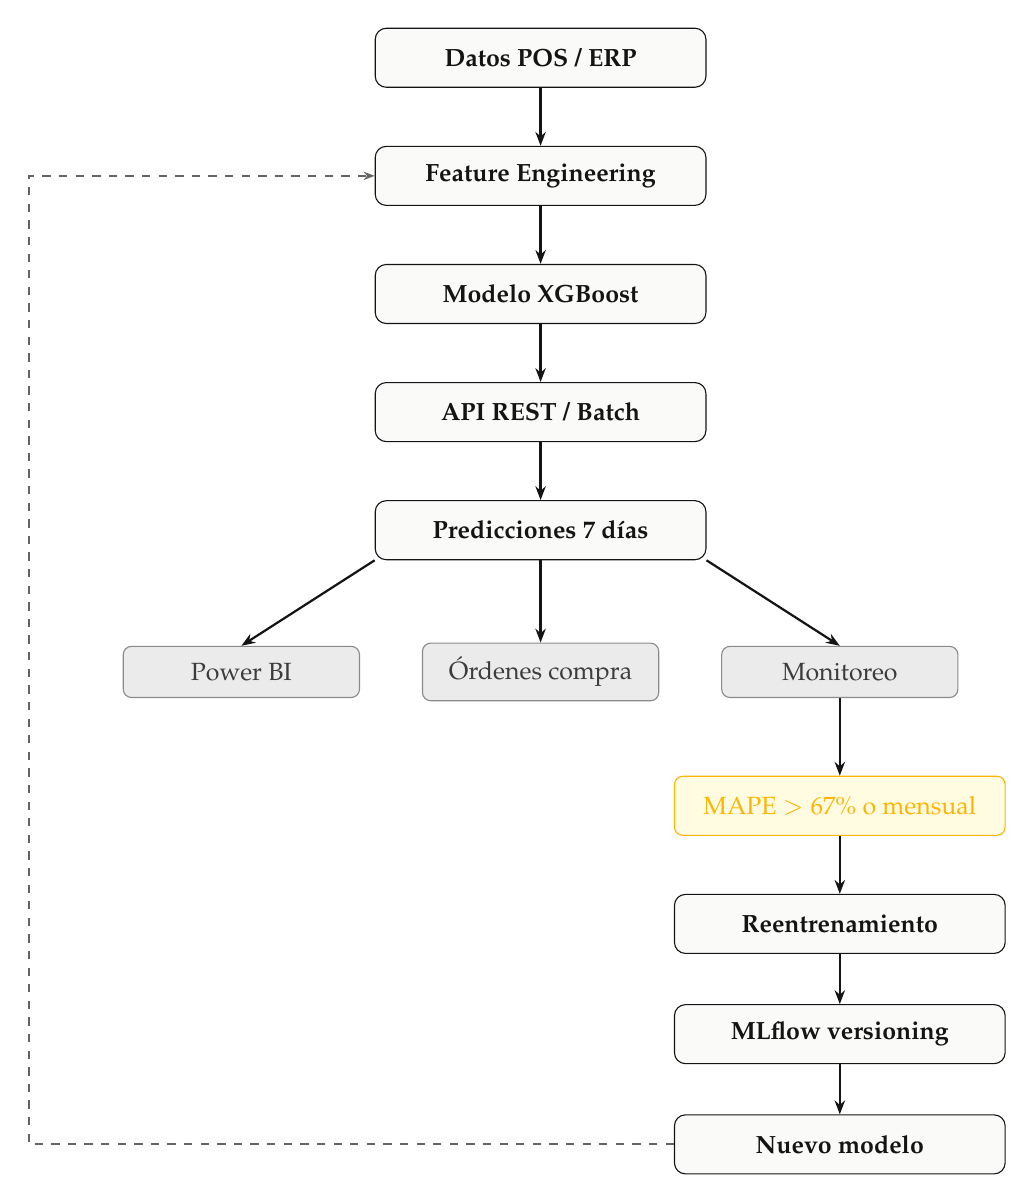
\begin{tikzpicture}[
  proc/.style={
    rectangle, rounded corners=4pt, draw=nuclioblue, fill=lightgray,
    minimum width=4.2cm, minimum height=0.75cm,
    align=center, font=\small\bfseries\color{nuclioblue}, inner sep=6pt
  },
  salida/.style={
    rectangle, rounded corners=3pt, draw=nucliolight!60, fill=nucliolight!10,
    minimum width=3.0cm, minimum height=0.65cm,
    align=center, font=\small\color{nucliolight}, inner sep=5pt
  },
  alerta/.style={
    rectangle, rounded corners=3pt, draw=accentorange, fill=rowalt,
    minimum width=4.2cm, minimum height=0.75cm,
    align=center, font=\small\color{accentorange}, inner sep=5pt
  },
  arr/.style={-{Stealth[length=5pt]}, thick, color=nuclioblue},
  darr/.style={-{Stealth[length=4pt]}, thick, dashed, color=nucliogray},
]

%% Pipeline principal
\node[proc]   (datos)   at (0,   0)    {Datos POS / ERP};
\node[proc]   (fe)      at (0,  -1.5)  {Feature Engineering};
\node[proc]   (modelo)  at (0,  -3.0)  {Modelo XGBoost};
\node[proc]   (api)     at (0,  -4.5)  {API REST / Batch};
\node[proc]   (pred)    at (0,  -6.0)  {Predicciones 7 d\'ias};

%% Salidas
\node[salida] (pbi)     at (-3.8, -7.8)  {Power BI};
\node[salida] (ord)     at ( 0,   -7.8)  {\'Ordenes compra};
\node[salida] (mon)     at ( 3.8, -7.8)  {Monitoreo};

%% Reentrenamiento
\node[alerta] (trigger) at (3.8, -9.5)   {MAPE $> 67\%$ o mensual};
\node[proc]   (retrain) at (3.8, -11.0)  {Reentrenamiento};
\node[proc]   (mlflow)  at (3.8, -12.4)  {MLflow versioning};
\node[proc]   (nuevo)   at (3.8, -13.8)  {Nuevo modelo};

%% Flechas
\draw[arr] (datos)  -- (fe);
\draw[arr] (fe)     -- (modelo);
\draw[arr] (modelo) -- (api);
\draw[arr] (api)    -- (pred);
\draw[arr] (pred.south west) -- (pbi.north);
\draw[arr] (pred.south)      -- (ord.north);
\draw[arr] (pred.south east) -- (mon.north);
\draw[arr] (mon)     -- (trigger);
\draw[arr] (trigger) -- (retrain);
\draw[arr] (retrain) -- (mlflow);
\draw[arr] (mlflow)  -- (nuevo);

%% Loop retroalimentacion: ruta explicita por el exterior izquierdo
\coordinate (lb) at (-6.5, -13.8);
\coordinate (lt) at (-6.5,  -1.5);
\draw[darr] (nuevo.west) -- (lb) -- (lt) -- (fe.west);

\end{tikzpicture}
\end{center}

% -
%  CAP\'ITULO 4 --- RESULTADOS Y CONCLUSIONES
% -
\chapter{Resultados y Conclusiones}

\section{Resultados del EDA}

Los seis hallazgos del an\'alisis exploratorio con implicaciones directas de negocio se resumen en la secci\'on de Metodolog\'{\i}a (el cap\'{\i}tulo anterior). Sus consecuencias operativas m\'as importantes son:

\begin{itemize}[leftmargin=*, noitemsep]
  \item New York lidera las ventas; las pol\'{\i}ticas de inventario no deben ser uniformes entre ciudades.
  \item El fin de semana genera entre un 27--33\% m\'as de ventas. Los pedidos deben planificarse para que el stock llegue antes del jueves.
  \item SUPERMARKET representa el 68,7\% de las ventas totales. Un fallo de stock en esta categor\'{\i}a tiene impacto desproporcionado.
  \item El gran pico de septiembre 2013 fue causado por una bajada agresiva de precios; confirma que las variables de precio son \textit{features} de alto valor predictivo.
  \item Los eventos especiales tienen impacto asim\'etrico: SuperBowl (+15,36\%), Easter (+12,38\%), Thanksgiving ($-$40,21\%).
  \item La autocorrelaci\'on en \textit{lag~1} es de 0,78 (ACF). El test ADF confirma que la serie es estacionaria ($p$-valor = 0,0008).
\end{itemize}

\section{Resultados del Clustering}

\subsection{Clustering de productos (k = 5)}

\textbf{\textit{Silhouette score}: 0,2249}. Los \textit{scores} por debajo de 0,25 son esperables en \textit{retail}: los productos de una misma cadena comparten muchos comportamientos de base (mismos d\'{\i}as de la semana, mismos eventos, misma estacionalidad), lo que reduce la separaci\'on natural entre cl\'usteres. La elecci\'on de k=5 se justifica por tener el mejor \textit{silhouette} y la mejor interpretabilidad de negocio.

\subsection{Clustering de tiendas (k = 3)}

\textbf{\textit{Silhouette score}: 0,2928}. Los \textit{scores} entre 0,25 y 0,30 indican diferencias comportamentales sutiles entre tiendas, lo cual es l\'ogico al pertenecer todas a la misma cadena y vender el mismo cat\'alogo.

La segmentaci\'on en 3 grupos permite:
\begin{itemize}[leftmargin=*, noitemsep]
  \item Priorizar el presupuesto de reposici\'on en las tiendas de mayor volumen.
  \item Aplicar estrategias diferenciadas de \textit{safety stock} seg\'un la variabilidad hist\'orica del cl\'uster.
\end{itemize}

\section{Comparativa de modelos predictivos}

Todos los modelos fueron evaluados sobre el mismo conjunto de test mediante RMSE.

\begin{table}[H]
  \centering
  \caption{Resultados comparativos de todos los modelos}
  \label{tab:modelos_full}
  \begin{tabularx}{0.8\textwidth}{L{5cm} C{3cm} C{3.5cm}}
    \toprule
    \rowcolor{headerblue}
    {\color{white}\textbf{Modelo}} &
    {\color{white}\textbf{RMSE (test)}} &
    {\color{white}\textbf{T.\ entrenamiento}} \\
    \midrule
    \rowcolor{white}   Baseline MA28      & 2,18 & --- \\
    \rowcolor{rowalt}  Ridge Regression   & 2,06 & $\sim$4 min \\
    \rowcolor{white}   Random Forest      & 2,01 & $\sim$34 min \\
    \rowcolor{rowalt}  CatBoost           & 1,98 & $\sim$56 min \\
    \rowcolor{white}   LightGBM           & 1,97 & $\sim$65 min \\
    \rowcolor{rowalt}  \textbf{XGBoost}   & \textbf{1,97} & \textbf{$\sim$24 min} \\
    \bottomrule
  \end{tabularx}
\end{table}

\textbf{Modelo ganador: \model{XGBoost}} con RMSE = 1,97, representando una \kpi{mejora del 9,6\%} sobre el baseline (de 2,18 a 1,97). El criterio definitorio entre XGBoost y LightGBM (ambos con RMSE = 1,97) fue la eficiencia computacional: XGBoost tard\'o $\sim$24 min frente a los $\sim$65 min de LightGBM, siendo $\sim$3$\times$ m\'as r\'apido con resultados equivalentes.

\subsection{Nota sobre el MAPE en validaci\'on (55,82\%)}

El MAPE obtenido sobre el conjunto de validaci\'on es del \textbf{55,82\%}, un valor que a primera vista parece elevado pero que es \textbf{esperado y normal} en problemas de \textit{forecasting retail} a nivel de granularidad \'{\i}tem-tienda-d\'{\i}a. La f\'ormula del MAPE,

\begin{equation}
  \text{MAPE} = \frac{1}{n} \sum_{i=1}^{n} \frac{|\hat{y}_i - y_i|}{y_i} \times 100
  \label{eq:mape}
\end{equation}

tiene en el denominador el valor real de ventas. Cuando las ventas son bajas (la mayor\'{\i}a de los registros corresponden a productos con 1--5 unidades diarias), dividir entre un n\'umero peque\~no infla el porcentaje aunque el error absoluto sea m\'{\i}nimo.

\begin{table}[H]
  \centering
  \caption{Resumen de m\'etricas del modelo final}
  \label{tab:metricas_final}
  \begin{tabularx}{0.88\textwidth}{L{4.5cm} C{2.5cm} X}
    \toprule
    \rowcolor{headerblue}
    {\color{white}\textbf{M\'etrica}} &
    {\color{white}\textbf{Valor}} &
    {\color{white}\textbf{Interpretaci\'on}} \\
    \midrule
    \rowcolor{white}   \textbf{RMSE}                   & \textbf{1,97} & El modelo se equivoca $\sim$2 unidades/d\'{\i}a; operativamente v\'alido \\
    \rowcolor{rowalt}  Mejora RMSE vs.\ baseline        & \textbf{+9,6\%}  & Supera al baseline; objetivo del proyecto cumplido \\
    \rowcolor{white}   MAPE (validaci\'on)               & 55,82\% & Inflado por baja rotaci\'on; no representativo como m\'etrica principal \\
    \rowcolor{rowalt}  \textbf{RMSE post-Optuna}        & \textbf{1,8994} & Mejora adicional tras optimizaci\'on bayesiana \\
    \rowcolor{white}   Mejora RMSE post-Optuna vs.\ baseline & \textbf{+13,1\%} & Supera ampliamente el objetivo m\'{\i}nimo del 5\% \\
    \bottomrule
  \end{tabularx}
\end{table}

\section{Importancia de variables (Feature Importance)}

\begin{table}[H]
  \centering
  \caption{Top 20 variables por importancia en el modelo XGBoost optimizado}
  \label{tab:feature_importance}
  \begin{tabularx}{\textwidth}{C{1.2cm} L{4.5cm} C{2.8cm} X}
    \toprule
    \rowcolor{headerblue}
    {\color{white}\textbf{Rank}} &
    {\color{white}\textbf{Feature}} &
    {\color{white}\textbf{Importance}} &
    {\color{white}\textbf{Interpretaci\'on}} \\
    \midrule
    \rowcolor{white}   1  & \code{sales\_rolling\_mean\_7}    & 1.606.980 & Predictor dominante; $\sim$4$\times$ el segundo \\
    \rowcolor{rowalt}  2  & \code{sales\_rolling\_mean\_14}   & 459.264   & Tendencia de 2 semanas \\
    \rowcolor{white}   3  & \code{sales\_rolling\_mean\_28}   & 72.202    & Tendencia mensual \\
    \rowcolor{rowalt}  4  & \code{sales\_lag\_1}              & 62.888    & Ventas de ayer \\
    \rowcolor{white}   5  & \code{sales\_rolling\_min\_28}    & 60.148    & Suelo de demanda del producto \\
    \rowcolor{rowalt}  6  & \code{is\_weekend}                & 34.955    & Efecto fin de semana \\
    \rowcolor{white}   7  & \code{store\_avg\_sales}          & 27.069    & Volumen base de la tienda \\
    \rowcolor{rowalt}  8  & \code{weekday\_int}               & 18.100    & Efecto d\'{\i}a-de-semana \\
    \rowcolor{white}   9  & \code{sales\_lag\_21}             & 17.582    & Memoria de 3 semanas \\
    \rowcolor{rowalt}  10 & \code{sales\_lag\_28}             & 17.520    & Memoria mensual \\
    \rowcolor{white}   11 & \code{price\_rolling\_mean\_4w}   & 14.627    & Precio medio reciente \\
    \rowcolor{rowalt}  12 & \code{item\_encoded}              & 12.854    & Identidad del producto \\
    \rowcolor{white}   13 & \code{quarter}                   & 12.320    & Estacionalidad trimestral \\
    \rowcolor{rowalt}  14 & \code{price\_lag\_1}              & 10.440    & Precio semana anterior \\
    \rowcolor{white}   15 & \code{month}                     & 9.225     & Granularidad mensual \\
    \rowcolor{rowalt}  16 & \code{year}                      & 9.071     & Tendencia interanual \\
    \rowcolor{white}   17 & \code{sales\_rolling\_std\_28}    & 9.048     & Volatilidad reciente \\
    \rowcolor{rowalt}  18 & \code{store\_encoded}             & 9.038     & Identidad de la tienda \\
    \rowcolor{white}   19 & \code{price\_ratio\_vs\_avg}      & 8.912     & Precio relativo a su media \\
    \rowcolor{rowalt}  20 & \code{item\_avg\_sales}           & 8.862     & Historial medio del producto \\
    \bottomrule
  \end{tabularx}
\end{table}

\textbf{Interpretaci\'on de negocio}: el modelo aprende principalmente de las \textbf{medias m\'oviles y \textit{lags} de ventas} (posiciones 1--5, 9--10 y 17 del \textit{ranking}), confirmando que el patr\'on hist\'orico reciente es el \textit{driver} principal de la demanda en \textit{retail}. El precio aparece en posiciones 11, 14 y 19, confirmando el hallazgo del EDA sobre la elasticidad precio-demanda.

\section{Sistema de reposici\'on de inventario}

\begin{table}[H]
  \centering
  \caption{Ejemplo de output del sistema de reposici\'on}
  \label{tab:replenishment}
  \begin{tabularx}{\textwidth}{L{3.5cm} L{2.2cm} C{2cm} C{2cm} C{2.5cm} C{1.5cm}}
    \toprule
    \rowcolor{headerblue}
    {\color{white}\textbf{item\_id}} &
    {\color{white}\textbf{store\_id}} &
    {\color{white}\textbf{cur.\ stock}} &
    {\color{white}\textbf{forecast\_7d}} &
    {\color{white}\textbf{order\_qty}} &
    {\color{white}\textbf{priority}} \\
    \midrule
    \rowcolor{white}   SUPERMARKET\_2\_194    & South\_End & 5      & 13,5 & $\sim$10 & \textbf{\color{red}ALTA} \\
    \rowcolor{rowalt}  SUPERMARKET\_3\_284    & South\_End & 1      & 2,0  & $\sim$1  & \textbf{\color{red}ALTA} \\
    \rowcolor{white}   HOME\_\&\_GARDEN\_2\_329 & South\_End & 3    & 4,0  & $\sim$1  & NORMAL \\
    \rowcolor{rowalt}  HOME\_\&\_GARDEN\_2\_314 & South\_End & 20--100 & 3,0 & 0       & NORMAL \\
    \rowcolor{white}   SUPERMARKET\_1\_049    & South\_End & 20--100 & 1,2 & 0        & NORMAL \\
    \rowcolor{rowalt}  HOME\_\&\_GARDEN\_1\_277 & South\_End & 20--100 & 53,7 & 0      & NORMAL \\
    \bottomrule
  \end{tabularx}
\end{table}

\section{Conclusiones finales}

\subsection{Conclusiones t\'ecnicas}

\begin{enumerate}[leftmargin=*, noitemsep]
  \item \textbf{El Gradient Boosting supera claramente a los modelos lineales} en este problema, confirmando la presencia de relaciones no lineales entre \textit{features} y ventas.
  \item \textbf{Las \textit{features} de \textit{lag} y las medias m\'oviles son las m\'as informativas}, validando la hip\'otesis de que los patrones temporales son el \textit{driver} principal de la demanda en \textit{retail}. \code{sales\_rolling\_mean\_7} domina con un \textit{importance score} $\sim$4$\times$ mayor que el segundo \textit{feature}.
  \item \textbf{XGBoost ofrece el mejor equilibrio entre rendimiento y eficiencia computacional} para este \textit{dataset} de $\sim$58M registros, siendo $\sim$3$\times$ m\'as r\'apido que LightGBM con resultados equivalentes.
  \item \textbf{La optimizaci\'on bayesiana (Optuna) confirm\'o que el modelo se beneficia de m\'as \'arboles y aprendizaje m\'as lento}: los par\'ametros \'optimos encontrados fueron \code{n\_estimators=1933} y \code{learning\_rate=0.023}. \code{max\_depth=8} alcanz\'o el l\'{\i}mite superior del rango de b\'usqueda, indicando que la complejidad extra est\'a justificada con 57M de filas.
  \item \textbf{El modelo generaliza bien y no est\'a sobreajustado}: el RMSE en el conjunto de validaci\'on (1,8994) es mejor que en el conjunto de test (1,9645).
  \item \textbf{El \textit{split} temporal estricto es fundamental} en problemas de series temporales para evitar \textit{data leakage} y obtener estimaciones realistas del rendimiento en producci\'on.
\end{enumerate}

\subsection{Conclusiones de negocio}

\begin{enumerate}[leftmargin=*, noitemsep]
  \item \textbf{El sistema reduce la incertidumbre de la gesti\'on de inventario}: el modelo final obtiene un \metric{RMSE = 1,8994} en el conjunto de validaci\'on, representando una \kpi{mejora del 13,1\%} sobre el \textit{baseline}, superando el objetivo m\'{\i}nimo del 5\%.
  \item \textbf{El sistema de abastecimiento automatiza una decisi\'on que hoy es manual}, liberando tiempo del equipo de operaciones y reduciendo el riesgo de error humano.
  \item \textbf{La segmentaci\'on por clustering permite estrategias diferenciadas}: no todos los productos y tiendas necesitan el mismo nivel de atenci\'on.
  \item \textbf{El proyecto es escalable}: la arquitectura desarrollada puede extenderse f\'acilmente a nuevos productos, tiendas o incluso cadenas del grupo.
\end{enumerate}

\section{Trabajo futuro}

\begin{table}[H]
  \centering
  \caption{\'Areas de mejora propuestas para iteraciones futuras}
  \label{tab:trabajo_futuro}
  \begin{tabularx}{\textwidth}{L{3cm} X}
    \toprule
    \rowcolor{headerblue}
    {\color{white}\textbf{\'Area}} &
    {\color{white}\textbf{Mejora propuesta}} \\
    \midrule
    \rowcolor{white}   \textbf{Datos}       & Integrar datos clim\'aticos (temperatura, lluvia) y de competencia (precios de competidores, aperturas de tiendas rivales) \\
    \rowcolor{rowalt}  \textbf{Modelos}     & Explorar modelos de series temporales espec\'{\i}ficos (Prophet, N-BEATS, Temporal Fusion Transformer) \\
    \rowcolor{white}   \textbf{Optuna}      & Ampliar el rango de b\'usqueda de \code{max\_depth} m\'as all\'a de 8, ya que el \'optimo encontrado alcanz\'o el l\'{\i}mite superior del rango actual \\
    \rowcolor{rowalt}  \textbf{FE}          & Recalcular las \textit{aggregate features} exclusivamente sobre el conjunto de \textit{train} para eliminar el \textit{data leakage} menor presente \\
    \rowcolor{white}   \textbf{Producci\'on}  & Refactorizar el c\'odigo del \textit{notebook} en m\'odulos Python independientes y \textit{containerizar} con Docker \\
    \rowcolor{rowalt}  \textbf{ERP}         & Integrar \code{current\_stock} en tiempo real desde el sistema ERP \\
    \rowcolor{white}   \textbf{Dashboard}   & Extender el dashboard de Power~BI con alertas autom\'aticas de \textit{stockout} \\
    \rowcolor{rowalt}  \textbf{Safety stock} & Calibrar \code{safety\_stock\_days} por cl\'uster de producto en lugar de usar un valor fijo global de 3 d\'{\i}as \\
    \bottomrule
  \end{tabularx}
\end{table}

% -
%  CAP\'ITULO 5 --- REFERENCIAS
% -
\chapter{Referencias Bibliogr\'aficas}

\noindent\textit{(Formato APA 7.\textordfeminine{} edici\'on, organizado por categor\'{\i}a tem\'atica.)}

\bigskip

\section*{Algoritmos y modelos}
\addcontentsline{toc}{section}{Algoritmos y modelos}

\begin{itemize}[leftmargin=2em, noitemsep]

\item Yandex. (s.f.). \textit{CatBoost documentation}. \url{https://catboost.ai/docs/}

\item Microsoft. (2025). \textit{LightGBM documentation}. \url{https://lightgbm.readthedocs.io/}

\item Optuna Contributors. (2018). \textit{Optuna documentation}. \url{https://optuna.readthedocs.io/}

\item XGBoost developers. (2025). \textit{XGBoost documentation}. \url{https://xgboost.readthedocs.io/}

\end{itemize}

\section*{Librer\'{\i}as de Python}
\addcontentsline{toc}{section}{Librer\'{\i}as de Python}

\begin{itemize}[leftmargin=2em, noitemsep]

\item NumPy Development Team. (2008--2026). \textit{NumPy documentation}. \url{https://numpy.org/doc/}

\item pandas Development Team. (2026). \textit{pandas documentation}. \url{https://pandas.pydata.org/docs/}

\item scikit-learn developers. (2007--2026). \textit{scikit-learn documentation}. \url{https://scikit-learn.org/stable/}

\end{itemize}

\section*{Dataset y competici\'on de referencia}
\addcontentsline{toc}{section}{Dataset y competici\'on de referencia}

\begin{itemize}[leftmargin=2em, noitemsep]

\item Makridakis Competitions. (2020). \textit{M5 Forecasting - Accuracy} [Dataset]. Kaggle. \url{https://www.kaggle.com/competitions/m5-forecasting-accuracy}

\item Makridakis, S., Spiliotis, E., \& Assimakopoulos, V. (2022a). The M5 competition: Background, organization, and implementation. \textit{International Journal of Forecasting}, \textit{38}(4), 1325--1336. \url{https://doi.org/10.1016/j.ijforecast.2021.07.007}

\item Makridakis, S., Spiliotis, E., \& Assimakopoulos, V. (2022b). M5 accuracy competition: Results, findings, and conclusions. \textit{International Journal of Forecasting}, \textit{38}(4), 1346--1364. \url{https://doi.org/10.1016/j.ijforecast.2021.10.009}

\end{itemize}

\section*{Metodolog\'{\i}a}
\addcontentsline{toc}{section}{Metodolog\'{\i}a}

\begin{itemize}[leftmargin=2em, noitemsep]

\item Dorard, L. (2015). \textit{The Machine Learning Canvas} (v1.0). \url{http://www.louisdorard.com/machine-learning-canvas}

\end{itemize}

% -
%  ANEXO --- ML CANVAS
% -
\renewcommand{\appendixname}{Anexo}
\appendix
\chapter{ML Canvas --- DSMarket}
\label{app:mlcanvas}

\begin{center}
{\large\bfseries\color{nuclioblue} OWNML Machine Learning Canvas}\\[0.3cm]
{\small Designed by: \textbf{Grupo 2} \quad|\quad Date: 05/03/2026 \quad|\quad Iteration: 1.2}\\[0.15cm]
{\footnotesize\color{nucliogray} Version 1.2. Created by Louis Dorard, Ph.D. Licensed under CC BY-SA 4.0. \url{https://ownml.co}}
\end{center}

\vspace{0.4cm}
\noindent El \textit{Machine Learning Canvas} es un marco estructurado para describir el ciclo completo de un sistema de ML en producci\'on. Se presentan a continuaci\'on los nueve bloques del \textit{canvas} aplicado al proyecto DSMarket.

\vspace{0.5cm}

%% ── BLOQUE 1: VALUE PROPOSITION ────────────────────────────────────────────
\begin{tcolorbox}[canvasbox, title={1.\ Value Proposition}]
\textbf{Beneficiario}: DSMarket (Compras, Operaciones, Direcci\'on).

\medskip
\textbf{Problema actual}: gesti\'on manual del inventario con dos costes cr\'iticos:
\begin{itemize}[noitemsep, leftmargin=*]
  \item \textit{Stockouts}: ventas perdidas y clientes insatisfechos.
  \item Exceso de stock: capital inmovilizado y productos obsoletos.
\end{itemize}

\medskip
\textbf{Soluci\'on ML}: pasar de una gesti\'on reactiva a una gesti\'on proactiva basada en datos, generando \'ordenes de reposici\'on autom\'aticas cada semana.

\medskip
\textbf{Valor esperado}: reducci\'on en \textit{stockouts} y exceso de stock. La cuantificaci\'on econ\'omica requiere datos operativos reales (stock actual, coste de almacenamiento, margen por producto) no disponibles en este proyecto acad\'emico.

\medskip
\textbf{Integraci\'on}: el \textit{pipeline batch} se ejecuta cada lunes a las 6:00~AM; resultados disponibles antes de las 8:00~AM para el departamento de compras.
\end{tcolorbox}

\vspace{0.4cm}

%% ── BLOQUE 2 + 3 lado a lado ────────────────────────────────────────────────
\noindent
\begin{minipage}[t]{0.485\textwidth}
\begin{tcolorbox}[canvasbox, title={2.\ Decisions}]
\textbf{Decisi\'on asistida}: el sistema genera autom\'aticamente \'ordenes de reposici\'on semanales.

\medskip
\textbf{Par\'ametros}:
\begin{itemize}[noitemsep, leftmargin=*]
  \item Horizonte: 7 d\'ias.
  \item Safety stock: \code{safety\_stock\_days = 3}.
  \item Prioridad \textbf{ALTA}: stock $< 0{,}5 \times$ punto reorden.
  \item Prioridad \textbf{NORMAL}: resto de casos.
\end{itemize}

\medskip
\textbf{Interfaces}: dashboard Power BI + fichero de \'ordenes exportado al ERP.

\medskip
\textbf{Explicabilidad}: Feature Importance publicada en el dashboard (\textit{top}: \code{rolling\_mean\_7}, \code{rolling\_mean\_14}, \code{rolling\_mean\_28}).
\end{tcolorbox}
\end{minipage}
\hfill
\begin{minipage}[t]{0.485\textwidth}
\begin{tcolorbox}[canvasbox, title={3.\ Prediction Task}]
\textbf{Tipo de tarea}: Aprendizaje supervisado --- Regresi\'on.

\medskip
\textbf{Entidad}: combinaci\'on \'item-tienda-d\'ia.

\medskip
\textbf{Variable objetivo}: \code{sales} --- unidades/d\'ia; valor continuo, no negativo, distribuci\'on asim\'etrica positiva.

\medskip
\textbf{Per\'iodo}: 29~ene~2011 -- 24~abr~2016 (1.913 d\'ias). Cobertura: 3.049 productos, 10 tiendas, 3 ciudades.

\medskip
\textbf{Modelos}: Baseline (MA28), Ridge, Random Forest, CatBoost, LightGBM, XGBoost.

\medskip
\textbf{Ganador}: XGBoost (RMSE = 1,97 pre-Optuna; 1,899 post-Optuna).
\end{tcolorbox}
\end{minipage}

\vspace{0.4cm}

%% ── BLOQUE 4 + 5 lado a lado ────────────────────────────────────────────────
\noindent
\begin{minipage}[t]{0.485\textwidth}
\begin{tcolorbox}[canvasbox, title={4.\ Impact Simulation}]
\textbf{M\'etrica principal}: RMSE (en unidades).\\
\textbf{M\'etrica secundaria}: MAPE.

\medskip
{\footnotesize\noindent
  Baseline (MA28): RMSE = 2,18\\[2pt]
  XGBoost pre-Optuna: RMSE = 1,97 \textbf{(+9,6\%)}\\[2pt]
  XGBoost post-Optuna: RMSE = 1,899 \textbf{(+13,1\%)}\\[2pt]
  MAPE validaci\'on: 55,82\%
}

\medskip
\textbf{Criterio despliegue}: RMSE$_{\text{nuevo}} <$ RMSE$_{\text{anterior}}$.\\
\checkmark\ Cumplido.

\medskip
\textbf{Rollback}: si RMSE$_{\text{nuevo}} \geq$ RMSE$_{\text{anterior}}$, se revierte autom\'aticamente.
\end{tcolorbox}
\end{minipage}
\hfill
\begin{minipage}[t]{0.485\textwidth}
\begin{tcolorbox}[canvasbox, title={5.\ Data Sources}]
Tres fuentes internas de DSMarket (2011--2016):

\medskip
\textbf{1.} \dataset{item\_sales.csv}\\
Ventas diarias formato \textit{wide}.\\
30.490 filas $\times$ 1.913 columnas.

\medskip
\textbf{2.} \dataset{daily\_calendar\_with\_events.csv}\\
Calendario con eventos especiales.

\medskip
\textbf{3.} \dataset{item\_prices.csv}\\
Precios semanales ($\sim$7M registros).

\medskip
Dataset consolidado (\textit{long}): $\sim$58,3M registros.

\medskip
\textbf{Origen}: M5 Forecasting (Kaggle, 2020), basado en datos reales de Walmart.
\end{tcolorbox}
\end{minipage}

\vspace{0.4cm}

%% ── BLOQUE 6: DATA COLLECTION (full width) ──────────────────────────────────
\begin{tcolorbox}[canvasbox, title={6.\ Data Collection}]
\begin{minipage}[t]{0.45\textwidth}
\textbf{Datos hist\'oricos}: extra\'idos de los sistemas internos de DSMarket para el per\'iodo 2011--2016.

\medskip
\textbf{Actualizaci\'on continua en producci\'on}:
\begin{itemize}[noitemsep, leftmargin=*]
  \item Ventas: diariamente desde el sistema POS.
  \item Precios: semanalmente desde el sistema de \textit{pricing}.
  \item Ambos flujos mediante ETL autom\'atico.
\end{itemize}
\end{minipage}
\hfill
\begin{minipage}[t]{0.50\textwidth}
\textbf{Etiquetado}: no requiere etiquetado manual; las ventas reales son el \textit{outcome} observado directamente.

\medskip
\textbf{Privacidad}: los datos no contienen informaci\'on personal (no aplica GDPR); son de uso interno.

\medskip
\textbf{Stock actual}: en el \textit{notebook} se simula con valores aleatorios. En producci\'on debe integrarse desde el ERP en tiempo real.
\end{minipage}
\end{tcolorbox}

\vspace{0.4cm}

%% ── BLOQUE 7 + 8 lado a lado ────────────────────────────────────────────────
\noindent
\begin{minipage}[t]{0.485\textwidth}
\begin{tcolorbox}[canvasbox, title={7.\ Features}]
{\small
\textbf{20 \textit{features}} en 4 categor\'ias:

\smallskip
\textbf{Lag} (m\'as importantes):
\begin{itemize}[noitemsep, leftmargin=*, topsep=1pt]
  \item \code{sales\_rolling\_mean\_7}, \code{\_14}, \code{\_28}
  \item \code{sales\_lag\_1}, \code{\_21}, \code{\_28}
  \item \code{sales\_rolling\_min\_28}, \code{\_std\_28}
\end{itemize}

\smallskip
\textbf{Producto/tienda}:
\code{store\_avg\_sales}, \code{item\_encoded}, \code{store\_encoded}, \code{item\_avg\_sales}.

\smallskip
\textbf{Temporales}:
\code{is\_weekend}, \code{weekday\_int}, \code{quarter}, \code{month}, \code{year}.

\smallskip
\textbf{Precio}:
\code{price\_rolling\_mean\_4w}, \code{price\_lag\_1}, \code{price\_ratio\_vs\_avg}.
}
\end{tcolorbox}
\end{minipage}
\hfill
\begin{minipage}[t]{0.485\textwidth}
\begin{tcolorbox}[canvasbox, title={8.\ Building Models}]
{\small
\textbf{Modelo en producci\'on}: XGBoost + Optuna (30 \textit{trials}, $\sim$46 min).

\medskip
\textbf{Hiperpar\'ametros \'optimos}:
\begin{itemize}[noitemsep, leftmargin=*, topsep=2pt]
  \item \code{n\_estimators}: 1.933
  \item \code{learning\_rate}: 0,023
  \item \code{max\_depth}: 8
  \item \code{min\_child\_weight}: 31
  \item \code{reg\_alpha}: 0,342
\end{itemize}

\medskip
\textbf{Reentrenamiento} (3 modalidades):
\begin{itemize}[noitemsep, leftmargin=*, topsep=2pt]
  \item Programado: mensual, \'ultimos 2 a\~nos.
  \item Por degradaci\'on: MAPE $> 67\%$ durante 2 semanas.
  \item Por evento estructural: nuevos productos/tiendas.
\end{itemize}

\medskip
\textbf{Versionado}: MLflow. Artefactos guardados:\\
\code{best\_model.pkl}, \code{label\_encoders.pkl},\\
\code{feature\_list.json}.

\medskip
\textbf{Split}: Train $\rightarrow$ Test $\rightarrow$ Validaci\'on.
}
\end{tcolorbox}
\end{minipage}

\vspace{0.4cm}

%% ── BLOQUE 9: MAKING PREDICTIONS ────────────────────────────────────────────
\noindent
\begin{minipage}[t]{0.485\textwidth}
\begin{tcolorbox}[canvasbox, title={9.\ Making Predictions}]
\textbf{Modo}: Batch (no \textit{real-time}).

\medskip
\textbf{Frecuencia}: cada lunes a las 6:00~AM.

\medskip
\textbf{Pipeline}: ETL $\rightarrow$ \code{build\_features.py} $\rightarrow$ \code{predict.py} $\rightarrow$ \dataset{replenishment\_orders.csv} $\rightarrow$ Power~BI.

\medskip
\textbf{Cobertura}: 10 tiendas $\times$ 3.049 productos = 30.490 registros.

\medskip
\textbf{Latencia aceptable}: $< 2$ horas para todo el cat\'alogo.

\medskip
\textbf{Artefactos}: \code{best\_model.pkl}, \code{label\_encoders.pkl}, \code{feature\_list.json}.
\end{tcolorbox}
\end{minipage}
\hfill
\begin{minipage}[t]{0.485\textwidth}
\begin{tcolorbox}[canvasbox, title={10.\ Monitoring}]
\textbf{Revisi\'on semanal} -- indicador implementado:

\medskip
\textbf{MAPE semanal por tienda}: alerta si $> 67\%$ (20\% de degradaci\'on sobre el 55,82\% actual). Acci\'on: investigar causa y decidir reentrenamiento.

\medskip
\textbf{RMSE \textit{rolling} (4 semanas)}: alerta si $> 2{,}36$ (20\% sobre RMSE = 1,97).

\medskip
\textbf{Trabajo futuro}: \textit{Stockout rate} real requiere integraci\'on con ERP. Una vez disponible, se podr\'ia ajustar \code{safety\_stock\_days} por cl\'uster de producto.

\medskip
\textbf{Trazabilidad}: todas las versiones del modelo registradas con m\'etricas, hiperpar\'ametros y artefactos.

\medskip
\textbf{Rollback autom\'atico}: si RMSE$_{\text{nuevo}} \geq$ RMSE$_{\text{anterior}}$.
\end{tcolorbox}
\end{minipage}

\vfill
\begin{center}
  \small\color{nucliogray}
  \rule{0.6\textwidth}{0.4pt}\\[4pt]
  Documento generado en el marco del TFM del M\'aster en Data Science --- Nuclio Digital School\\
  Versi\'on 1.0 --- Marzo 2026
\end{center}

\end{document}
